\section{Nedscript-Validierung}

Zur Validierung von Ned-Skripten sollte eine Lua-Bibliothek
geschrieben werden, deren API äquivalent zur der von Ned bereit gestellten ist
und Ausführung von Ned-Skript ,,Dry-Runs'' ohne das Booten einer Fiasco.OC
Instanz und Starten von Moe und Ned ermöglicht.
Dadurch kann beim Debuggen fehlerhafter Ned-Skripte Zeit eingespart werden.

Die Funktionen der Bibliothek registrieren Ressourcen und Kommunikations-Kanäle,
die bei tatsächlicher Ausführung des Skriptes allokiert werden würden, und
prüfen diese teilweise auf Plausibilität.

Außerdem können die allokierten Kernel-Objekte, gestarteten Programme und die
zwischen ihnen bestehenden hierarchischen Beziehungen und (transitiven)
Kommunikationskanäle (über IPC Capabilities, geteilten Speicher etc.) über ein
breites Spektrum an Optionen konfigurierbar im \textit{Graphviz} Datenformat
ausgegeben werden. Dies ermöglicht eine schnelle visuelle Überprüfung der
Korrektheit der durch ein Ned-Skript erzeugten Programmbeziehungen.

Es wurden letztendlich zwei unabhängige Varianten der Bibliothek entwickelt.
Die erste implementiert die genannten Funktionen indem lediglich der in C++
verfasste Teil von Ned durch Lua Code erstzt und mit dem bereits in Lua
verfassten Teil von Ned integriert wird. Die zweite wurde von Grund auf (d.h.
komplett unabhängig von der existierenden Ned-Implementierung) geschrieben.
Hieraus ergab sich die Möglichkeit, die bestehende Ned-Dokumentation durch
Vergleich des Verhaltens beider Versionen auf Fehler und Unklarheiten zu
untersuchen.

Abbildung~\ref{fig:nedmock} zeigt beispielhaft den für
\texttt{l4re\_ipc\_example.cfg} aus Listing~\ref{lst:l4re_ipc_example_ned}
erzeugten Kommunikations-Graphen. Die schwarzen Pfeile zeigen an, dass beide
Programme unter dem Namen \texttt{cap} Zugriff auf die gleiche IPC Gate
Capability haben.  Der rote Pfeil zeigt an, dass ein unidirektionaler
Kommunikationskanal von \texttt{l4re\_ipc\_example\_sender} zu
\texttt{l4re\_ipc\_example\_receiver} besteht.

\begin{figure}
  \centering
  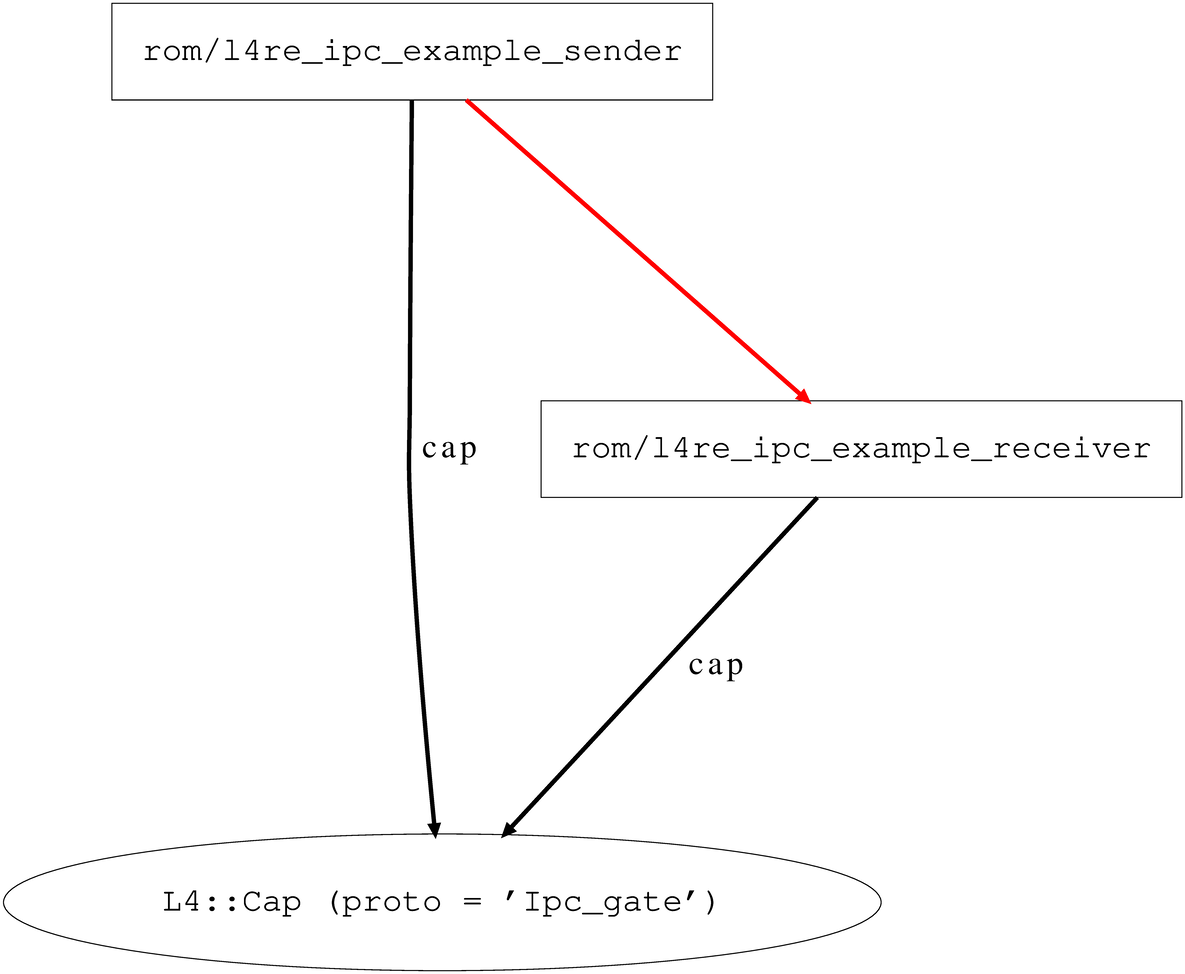
\includegraphics{../resources/nedmock.png}
  \caption{Kommunikations-Struktur von \texttt{l4re\_ipc\_example.cfg}}
  \label{fig:nedmock}
\end{figure}
